\documentclass[conference]{IEEEtran}
\usepackage{natbib}
\usepackage{amsmath,amssymb,amsfonts}
\usepackage{algorithmic}
\usepackage{hyperref}
\usepackage[capitalize,nameinlink]{cleveref}
\usepackage[italicdiff]{physics}
\usepackage{graphicx}
\usepackage{textcomp}
\usepackage{xcolor}

\DeclareMathOperator\sign{sign}

\begin{document}

\title{Building a Physical Pendulum}

\author{\IEEEauthorblockN{Brian Shimanuki}
\IEEEauthorblockA{bshimanuki@mit.edu}
}

\maketitle

\begin{abstract}
	I built the physical pendulum with a controller to stabilize at the unstable fixed point. The main goals of this project are to explore the characteristics which must be considered in real systems rather than in our idealized models from class. The single pendulum uses an energy-shaping swing up controller followed by a LQR controller once the region of convergence has been reached.

	I also control a double pendulum to reach and stabilize at the highest potential energy fixed point in pydrake. I built the components for a physical double pendulum, but could not read the state correctly when the chaotic second arm moves at high speeds.

	Code and files (including videos) can be found at \url{https://github.com/bshimanuki/double-pendulum}.
\end{abstract}

\section{Introduction}
The pendulum is a classical system with nonlinear mechanics. When the joint has input torque limits, the system is underactuated but is still controllable. I built my own actuated pendulum with a controller to stabilize at the unstable fixed point.

The double pendulum (often called the Pendubot) has more complex mechanics. Despite being underacted, the double pendulum is controllable with a single actuator at the shoulder and can stabilize in the inverted position as in \cref{fig:inverted_double_pendulum}. My original plan was to build and stabilize a double pendulum with a single actuator, and I built the system, but could not capture changes in the state quickly enough in the reduced code I was using. However, I use a cascade of controllers to bring the double pendulum to the upright position in simulation using pydrake, following the strategy of \cite{albahkali} in swinging each link up one at a time.

This project was worthwhile to grasp the challenges of building and designing control for a physical system. There is benefit to putting everything in action even on a simple pendulum.

\begin{figure}[h]
	\centering
	\includegraphics[width=4in]{double_pendulum_rotary.png}
	\caption{Double pendulum with single actuator at the top.}
	\label{fig:double_pendulum}
\end{figure}

\begin{figure}[h]
	\centering
	\includegraphics[width=3in]{inverted_double_pendulum_rotary.png}
	\caption{Inverted double pendulum.}
	\label{fig:inverted_double_pendulum}
\end{figure}

\section{Background}
The pendulum and double pendulum are well studied systems which have a variety of controllers. Many of the simplest controllers rely on energy-shaping swing up phases followed by a stabilization phase. Spong and Block\cite{spong} used LQR to stabilize the double pendulum at the inverted position and Fantoni et.\ al.\cite{fantoni} proposed an energy-shaping controller to solve the swing up phase.

Albahkali et.\ al\cite{albahkali} splits the swing up into separate energy-shaping maneuvers to first bring the first link to the inverted position and then bring the second link also to the inverted position while keeping the first link close to its top.

I implemented a similar strategy to \cite{albahkali} in to bring the double pendulum to the inverted position in simulation.

\section{System Dynamics}
The double pendulum has two connected arm links with an actuated shoulder joint and a free elbow joint. The relevant parameters, state variables, and forces are shown in \cref{fig:pendubot}. Note that the single pendulum can be thought of as a special case of the double pendulum where the second arm has no mass or length (though this formulation does not work for LQR since there are singular matrices).

\begin{figure}[ht]
	\centering
	\includegraphics[width=2in]{pendubot.png}
	\caption{The double pendulum. Image modified from the Acrobot in \cite{tedrake}.}
	\label{fig:pendubot}
\end{figure}

The dynamics can be described with the manipulator equations
\begin{equation}
	M\ddot q+C\dot q = \tau_g+Bu \\
\end{equation}
with $M$, $C$, $\tau_g$, and $B$ as in \cref{fig:matrices}.
\begin{figure*}
	\begin{align}
		M &= \begin{bmatrix}
			I_1+I_2+m_2l_1^2+2m_2l_1l_{c2}\cos\theta_2 & I_2+m_2l_1l_{c2}\cos\theta_2 \\
			I_2+m_2l_1l_{c2}\cos\theta_2 & I_2
		\end{bmatrix} \\
		M^{-1} &= \frac1{I_1I_2+m_2l_1^2I_2-m_2^2l_1^2l_{c2}^2\cos^2\theta_2} \begin{bmatrix}
			I_2 & -I_2-m_2l_1l_{c2}\cos\theta_2 \\
			-I_2-m_2l_1l_{c2}\cos\theta_2 & I_1+I_2+2m_2l_1l_{c2}\cos\theta_2
		\end{bmatrix} \\
		C &= \begin{bmatrix}
			-2m_2l_1l_{c2}\dot\theta_2\sin\theta_2 & -m_2l_1l_{c2}\dot\theta_2\sin\theta_2 \\
			m_2l_1l_{c2}\dot\theta_1\sin\theta_2 & 0
		\end{bmatrix} \\
		\tau_g &= \begin{bmatrix}
			-m_1gl_{c1}\sin\theta_1-m_2g(l_1\sin\theta_1+l_{c2}\sin(\theta_1+\theta_2)) \\
			-m_2gl_{c2}\sin(\theta_1+\theta_2)
		\end{bmatrix} \\
		B &= \begin{bmatrix}
			1 \\ 0
		\end{bmatrix} \\
		\ddot q &= M^{-1}(\tau_g + Bu - C\dot q) \\
	\end{align}
	\caption{Matrices for the manipulator equation.}
	\label{fig:matrices}
\end{figure*}

Working through the feedback linearization, we can solve for linearized matrices $A_{lin}$ and $B_{lin}$ at the upright fixed point. A more complete derivation is shown in the appendix.
\begin{align}
	x &= \begin{bmatrix}
		\theta_1 \\ \theta_2 \\ \dot \theta_1 \\ \dot \theta_2
	\end{bmatrix} \\
	A_{lin} &= \begin{bmatrix}
		O_2 & I_2 \\
		M^{-1}\frac{\partial\tau_g}{\partial q} & O_2
	\end{bmatrix}_{x=x_f,u=u_f} \\
	B_{lin} &= M^{-1}B \\
	\dot x &\approx A_{lin}x + B_{lin}u
\end{align}
$x_f$ and $u_f$ are the state and input at the upright fixed point.

These are used for the LQR controller by solving the Riccati equation.

\section{Controllers}
My controller has three phases. The first energy shaping swing up controller for the first arm. The second is an energy-shaping swing up controller for the second arm that keeps the first arm close to the inverted position. The final phase is LQR stabilization.

\subsection{First Swing up}
The first swing up controller applies a torque in the direction that will increase the energy fo the system.

The energy of the system can be formulated as
\begin{align}
	E(q,\dot q) &= \frac12 (\dot q^TM\dot q + (m_1l_{c1}+m_2l_1)g(-\cos q_1) \\
	&\qquad + m_2l_{c2}g(-\cos(q_1+q_2))) \\
	\frac{\partial^2 E}{\partial t\partial u}(q,\dot q) &= \frac12 (M^{-1}BM\dot q + \dot q^TB)
\end{align}

Let $x_f$ be the upright fixed point and let $\bar q_1=q_1-\pi$. My swingup controller applies a torque
\begin{equation}
	\tau(x) = -K_{e_1} (E(x) - E(x_f)) - K_q \bar q_1 - K_v v_2
\end{equation}
.

\subsection{Second Swing Up}
The second swing up phase keeps the first arm link within $\alpha$ of the upright and shapes the energy of the second link. It sums the torque required to counteract all other torques on the first link along with a driven torque to give the second link energy. It has constraints on the output torque when the energy threshold is reached or when $q_1$ exceeds $\alpha$ but otherwise drives in the direction of the undriven $a=M^{-1}(-C\dot q+\tau_G)$.

As described in \cite{albahkali}, a hard braking torque will transfer the velocity of $v_1$ to $v_2$ such that $\tilde v_1=0$ and $\tilde v_2=v_2 + (1+\frac{l_1\cos(q_2)}{l_{c2}})v_1$ where $\tilde v_1$ and $\tilde v_2$ are the velocities after braking.

The controller is implemented as follows. If $E(\tilde x)>E(x_f)$ (ie.\ braking hard would reach the energy of the upright), set $\tau = -K_w\sign(v_1)$. Else, if $|\bar q_1| > \alpha$ and $q_1$ and $v_1$ have the same sign, $\tau=-K_w\sign(v_0)$ to keep the first link approximately within $\alpha$. Else, set $\tau=K_{e_2}\sign{a_1+a_2}(E(\tilde x)-E(x_f))$.

\subsection{LQR}
An LQR controller is used near the top to stabilize the system. $A_{lin}$ and $B_{lin}$ are taken from above. It is useful to think about the cost in terms of $\theta_1$ and $\theta_1+\theta_2$. Define
\begin{equation*}
	R^{*} = \begin{bmatrix}
		1 & 0 & 0 & 0 \\
		1 & 1 & 0 & 0 \\
		0 & 0 & 1 & 0 \\
		0 & 0 & 1 & 1
	\end{bmatrix}
\end{equation*}

I use $R=[0.1]$ and $Q = R^{*T}Q'R$ with
\begin{equation*}
	Q^{*} = \begin{bmatrix}
		10 & 0 & 0 & 0 \\
		0 & 200 & 0 & 0 \\
		0 & 0 & 10 & 0 \\
		0 & 0 & 0 & 80
	\end{bmatrix}
\end{equation*}
.

Together these controllers are tuned for gains and phase switching conditions and have been used to invert and stabilize a double pendulum in pydrake.

\section{Hardware Description}

I built a pendulum and double pendulum as shown in \cref{fig:build}. It is held up by a frame. On the top, a motor provides actuation as the control input for the system. The arms are laser cut from acrylic. Each arm has arc segments cut out from the acrylic to form an optical encoder on one end as shown \cref{fig:rotary}. This is read by the reflectance from an IR LED emitter to an IR diode receiver.

\begin{figure}[ht]
	\centering
	\includegraphics[width=3in]{build.jpg}
	\caption{The build of the double pendulum.}
	\label{fig:build}
\end{figure}

\begin{figure}[ht]
	\centering
	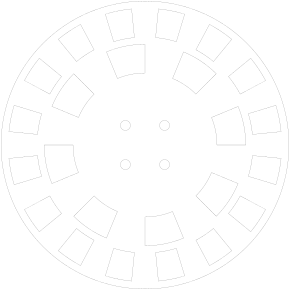
\includegraphics[width=1.5in]{rotary.jpg}
	\includegraphics[width=1.5in]{led.jpg}
	\caption{Laser cut rotary encoder and IR pairs.}
	\label{fig:rotary}
\end{figure}

The IR receiver diodes are read by a microcontroller which tracks the state as a 3 bit gray code. The rotary encoder has 128 positional states, so the gray code repeats every 8 steps. This means that at least one of every third step must be scanned or else the read state will be off by a multiple of 8. This is contributed to the limiting factor which prevented me from controlling the double pendulum.

The angular velocity is computed using the time interval between reading successive states. Together, the positional and angular velocities are sent to the controller to compute the desired signal, which is applied to a DC motor with pulse width modulation.

\section{Difficulties in the Build}
\subsection{Latency}
Real systems have latency, which is unmodeled in the simulation we have done in class. With this project, the latency of my system is approximately 2ms, which was negligible for the single pendulum dynamics. However, it was certainly a constant factor in my degin considerations.

\subsection{Friction}
Physical components have friction. Ball bearings can help with rotating components, but friction always exists. The first motor I tried using was a gearhead motor, which has enough internal friction to almost stop the pendulum at the base in the initial swing when dropped. I switched to a different DC motor without gears, which worked a lot better.

\subsection{Time Scales of Electronic Components}
With the circuitry I set up, the LED diode receivers could only measure signals at a max of around 400Hz. This was sufficient for the single pendulum, but the double pendulum exceeded this with the precision of the rotary encoders I was using. This prevented me from being able to read the correct state for the double pendulum.

\section{Summary of Results}
\subsection{Single Pendulum}
I could swing up and stabilize the physical single pendulum. It had a single swing up phase and then a stabilization phase.

\begin{figure}[ht]
	\centering
	\includegraphics[width=3in]{scope.jpg}
	\caption{Debugging information output to an oscilloscope showing $\theta$ on top and $u$ on the bottom for the physical single pendulum swinging up and stabilizing.}
	\label{fig:scope}
\end{figure}

\subsection{Double Pendulum}
I can swing up and stabilize the double pendulum in simulation using pydrake with the approach described in the previous sections. However, I was not able to start with the controls on the physical double pendulum because the state changes too fast for my sensors to detect correctly.

\section{Future Work}
The next steps for being able to perform control on the double pendulum is to remake the rotary encoder for the second arm link. I would need to have addition rings of holes and LED pairs to encode the positional state with more than 3 bits. Once I can consistently keep track of the state of the pendulum across some of the chaotic motions of the double pendulum, I can start tuning the controls.

\section{Conclusion}
Physical systems have many characteristics which are not present in simplified models. Seeing how far I could get with designing an underactuated system and control it has been enlightening. Even achieving success on the single pendulum has been very worthwhile.

\nocite{*}
\bibliographystyle{plain}
\bibliography{references}

\onecolumn
\section*{Appendix}
\subsection*{Feedback Linearization Derivation}
\begin{align}
	M^{-1} &= \frac1{I_1I_2+m_2I_1^2I_2-m_2^2l_1^2l_{c2}^2\cos^2\theta_2} \begin{bmatrix}
		I_2 & -I_2-m_2l_1l_{c2}\cos\theta_2 \\
		-I_2-m_2l_1l_{c2}\cos\theta_2 & I_1+I_2+2m_2l_1l_{c2}\cos\theta_2
	\end{bmatrix} \\
	M^{-1}_{q_1=\pi,q_2=0} &= \frac1{I_1I_2+m_2I_1^2I_2-m_2^2l_1^2l_{c2}^2} \begin{bmatrix}
		I_2 & -I_2+m_2l_1l_{c2} \\
		-I_2+m_2l_1l_{c2} & I_1+I_2-2m_2l_1l_{c2}
	\end{bmatrix} \\
	\frac{\partial\tau_g}{\partial q} &= \begin{bmatrix}
		-m_1gl_{c1}\cos\theta_1 - m_2g(l_1\cos\theta_1+l_{c2}\cos(\theta_1+\theta_2)) & -m_2gl_{c2}\cos(\theta_1+\theta_2) \\
		-m_2gl_{c2}\cos(\theta_1+\theta_2) & -m_2gl_{c2}\cos(\theta_1+\theta_2) \\
	\end{bmatrix} \\
	\frac{\partial\tau_g}{\partial q}_{q_1=\pi,q_2=0} &= \begin{bmatrix}
		m_1gl_{c1} + m_2g(l_1+l_{c2}) & m_2gl_{c2} \\
		m_2gl_{c2} & m_2gl_{c2} \\
	\end{bmatrix} \\
	\frac{\partial\tau_g}{\partial q}_{q_1=\pi,q_2=0} &= \begin{bmatrix}
		m_1gl_{c1} + m_2gl_1 & 0 \\
		0 & 0 \\
	\end{bmatrix} + m_2gl_{c2} \\
	\dot x &= \begin{bmatrix}
		\dot q \\
		M^{-1}(\tau_g+Bu-C\dot q)
	\end{bmatrix} \\
	\dot x &\approx A_{lin}(x-x^*) + B_{lin}(u-u^*) \\
	A_{lin} &= \begin{bmatrix}
		O_2 & I_2 \\
		M^{-1}(\frac{\partial\tau_g}{\partial q} + \frac{\partial B}{\partial q}u) & O_2
	\end{bmatrix}_{x=x^*,u=u^*} \\
	A_{lin} &= \begin{bmatrix}
		O_2 & I_2 \\
		M^{-1}\frac{\partial\tau_g}{\partial q} & O_2
	\end{bmatrix}_{x=x^*,u=u^*} \\
	B_{lin} &= M^{-1}B \\
\end{align}

\end{document}
